    \item A circular insulated copper wire loop is twisted to form two loops of area A and 2A as shown in the figure. At the point of crossing the wires remain electrically insulated from each other. The entire loop lies in the plane (of the paper). A uniform magnetic field \( \vec{B} \) points into the plane of the paper. At \( t = 0 \), the loop starts rotating about the common diameter as axis with a constant angular velocity \( \omega \) in the magnetic field. Which of the following options is/are correct?\begin{center}
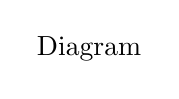
\begin{tikzpicture}
\node {Diagram};
\end{tikzpicture}
\end{center}
        \begin{tasks}(1)
            \task The emf induced in the loop is proportional to the sum of the areas of the two loops
            \task The amplitude of the maximum net emf induced due to both the loops is equal to the amplitude of maximum emf induced in the smaller loop alone
            \task The net emf induced due to both the loops is proportional to \( \cos \omega t \)
            \task The rate of change of the flux is maximum when the plane of the loops is perpendicular to plane of the paper
        \end{tasks}
